\documentclass[12pt]{article}         
\usepackage{fullpage}
\usepackage[shortlabels]{enumitem}
\usepackage{amsmath}
\usepackage{amsfonts}

\usepackage{graphicx}
\graphicspath{ {./images/} }

\usepackage{listings}
\usepackage{color}

\definecolor{dkgreen}{rgb}{0,0.6,0}
\definecolor{gray}{rgb}{0.5,0.5,0.5}
\definecolor{mauve}{rgb}{0.58,0,0.82}

\lstset{frame=tb,
  language=Java,
  aboveskip=3mm,
  belowskip=3mm,
  showstringspaces=false,
  columns=flexible,
  basicstyle={\small\ttfamily},
  numbers=none,
  numberstyle=\tiny\color{gray},
  keywordstyle=\color{blue},
  commentstyle=\color{dkgreen},
  stringstyle=\color{mauve},
  breaklines=true,
  breakatwhitespace=true,
  tabsize=3
}

%\usepackage{amsmath}
%\usepackage{amssymb}
%\usepackage{enumitem}

\title{CS250 Homework $\#$4}
\author{Sean O'Dea \footnote{Collaborated with Tomas Acu\~na}}

\begin{document}
\maketitle

\section*{\textbf{1: P4.4.7} [12 pts]}
A polygon is called \textbf{convex} if every line segment from one vertex to another lies entirely within the polygon. To \textbf{triangulate} a polygon, we take some of these line segments, which don’t cross one another, and use them to divide the polygon into triangles. Prove, by strong induction for all naturals $n$ with $n \geq 3$, that every convex polygon with $n$ sides has a trian-gulation, and that every triangulation contains exactly $n - 2$ triangles. (\textbf{Hint}: When you divide an $n$-gon with a single line segment, you create an $i$-gon and a $j$-gon for some naturals $i$ and $j$. What does your strong inductive hypothesis tell you about triangulations of these polygons?)


\subsection*{\textbf{Solution:}}
Proof by Induction:\\

Base Case:
$n = 3$; A polygon with 3 sides (a triangle) contains no lines for its triangulation. It contains one triangle. $3-2=1$ so the condition is satisfied.\\

Inductive Hypothesis: Assume for any arbitrary natural $k \geq 3$, all convex polygons with $\leq k$ sides can be triangulated into exactly $k-2$ triangles.\\

Inductive Step: We can derive from the hypothesis that adding a side to the polygon should add 1 triangle to its triangulation.
\[ k \text{ sides} \iff k-2 \text{ triangles} \]
\[ k+1 \text{ sides} \iff k-1 \text{ triangles} \]
By its geometric definition, a polygon must have the same number of sides as it has points. This implies that if we add a point to a polygon with $k$ sides it will have now have $k+1$ sides.
If we add a point outside of the polygon and connect it to the two closest points to itself with line segments (in a way such that our convex property is not violated) we now have a polygon with $k+1$ sides. Not only that but the region now enclosed by the three newly connected points constructs a triangle (in addition to the previously triangulated shape). The line that was formerly an edge is now contained inside the polygon, and does not intersect with the other triangulation dividers.

\begin{figure}[h]
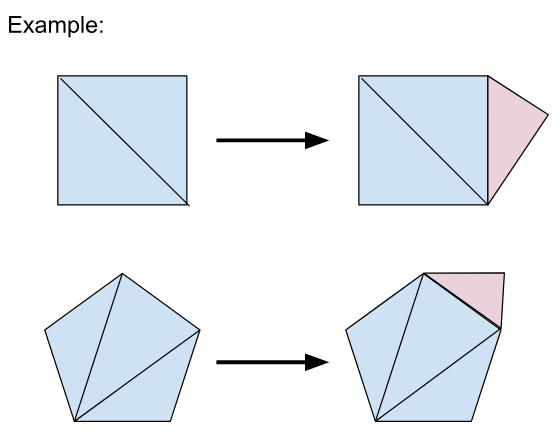
\includegraphics[width=8cm]{drawing}
\centering
\end{figure}

We can now conclude that adding a side to the polygon adds one additional triangle to the triangulation. $k+1 \text{ sides} \iff k-1 \text{ triangles}$. We can also conclude a triangulation exists for all polygons because if the triangulation exists for an arbitrary polygon with number of sides $k$ $(\geq 3)$ we know it also exists for the polygon created by adding a point ($k+1$ sides).\\

*Note the fact that we can reach any given convex polygon by adding points in the manner above to the correct preliminary polygon. We're allowed to to do this because of the strong induction stating the hypothesis is true for all polygons of less sides. (This is to clear up any confusion that this only proves the case for the polygons that can specifically be reached by adding points onto a specified base case triangle. We can theoretically start with any triangle we want and add points to it.)


\newpage
\section*{\textbf{2: P4.7.6} [12 pts]}
(uses Java) We can define the \textbf{balanced parenthesis language} using recursion. This is the set of sequences of left and right parentheses that are balanced, in that every left paren has a matching right paren and the pairs are nested properly. We’ll use “$L$” and “$R$” instead of “(” and “)” for readability. \\
We define the language Paren by the following four rules:

\begin{enumerate}
    \item $\lambda$ is in Paren.

    \item If $u$ is in Paren, then so is $LuR$.

    \item If $u$ and $v$ are in Paren, then so is $uv$.

    \item No other strings are in Paren.
\end{enumerate}

\noindent
Write a real-Java static method (or a Python function) \texttt{isBalanced} that takes a \texttt{String} argument and returns a \texttt{boolean} telling whether the input string is in Paren. A non-recursive method is simpler.

\subsection*{\textbf{Solution:}}
\begin{lstlisting}
public static boolean isBalanced(String s) {
	if (s.isEmpty()) return true;
	int L = 0;
	int R = 0;
	for (int i = 0; i < s.length(); i++){
		char c = s.charAt(i);
		if (c == '(') L++;
		if (c == ')') R++;
	}
	return L==R;
}
\end{lstlisting}


\newpage
\section*{\textbf{3: P4.9.2} [10 pts]}
Prove that any directed cycle in the graph of a partial order must only involve one node. (\textbf{Hint:} If the cycle were to contain two distinct nodes $x$ and $y$, what does transitivity tell you about arcs between $x$ and $y$?)


\subsection*{\textbf{Solution:}}
Let's say we have an arbitrary directed graph $G$ of a partial order. Let's assume $G$ has a directed cycle including at least the distinct nodes $x$ and $y$. By the Transitivity Theorem, there exists a path between all nodes in this cycle, meaning the nodes in the cycle are strongly connected. $x$ and $y$ must be strongly connected, thus there exists a path from $x$ to $y$ and a path from $y$ to $x$. This would violate the antisymmetry of a partial order relation and so we have a contradiction.\\\\
\noindent
The only cycle that can exist in a directed graph of a partial order is the trivial cycle only containing one node. 


\newpage
\section*{\textbf{4: P4.10.5} [10 pts]}
Prove that if $T$ is any rooted directed binary tree (where every internal node has out-degree exactly two), then the number of leaves in $T$ is one greater than the number of internal nodes. (\textbf{Hint:} Use induction on the definition of such trees.)



\subsection*{\textbf{Solution:}}
Note: Assume all trees discussed here have internal nodes with a degree of exactly two.\\
\noindent
Proof by Induction:\\

Base Case: A rooted directed binary tree with a single node (height $h=0$) has 0 internal nodes and 1 leaf.\\

Inductive Hypothesis: Assume for all rooted directed binary trees with a height $h \leq n$, the number of interal nodes is ones less than the number of leaves.\\

Inductive Step: We can construct a new tree $T$ with root node $r$ and left and right subtrees $T_1$ and $T_2$ of height $h \leq n$. Let's call the number of internal nodes in the left subtree $I_1$ and in the right $I_2$. From our hypothesis we know the subtrees have the property described above meaning we can represent the number of leaves in the left and right subtrees as $I_1 + 1$ and $I_2 + 1$.\\

For our newly constructed tree $T$ (the height of which is at least one larger than the heights of either subtree) the number of nodes will be the the internal nodes of the left subtree and internal nodes of the right subtree, plus the root which will also be internal. Totaled this is
\[ I_1 + I_2 + 1 \]
The total number of leaves will be the number of leaves in the left and right subtrees or
\[ I_1 + 1 + I_2 + 1 = I_1 + I_2 + 2\]
We can now see the total number of leaves is equal to
\[ (I_1 + I_2 + 1) + 1\]
And so the number of leaves will be one greater than the number of internal nodes for any rooted directed binary tree with internal nodes of degree 2.


\newpage
\section*{\textbf{5: P4.11.1} [12 pts]}
Show that a $3 \times n$ rectangle can be covered exactly with L-shaped tiles if and only if $n$ is even. (\textbf{Hint:} For the negative result, use induction on all odd numbers and an indirect proof in the inductive step.)


\subsection*{\textbf{Solution:}}
Proof by Induction on Evens:\\
In this case we will only deal with the evens so we'll have a $3 \times 2k$ rectangle where $k$ is some natural.\\

Base Case: $k=1$, a $3 \times 2$ rectangle can be tiled by two L-shaped tiles on opposite corners.
\begin{figure}[h]

\includegraphics[width=2cm]{3x2}
\centering
\end{figure}
\\
\indent
Inductive Hypothesis: Assume any rectangle of dimension $3 \times n$, where $n$ is even and $\leq 2k$, can be covered exactly with L-shaped tiles.\\

Inductive Case: Let's say we have some arbitrary rectangle of dimension $3 \times 2k$. We know this rectangle can be fully covered by our hypothesis. If we then consider a rectangle with dimension $3 \times 2(k+1) = 3 \times (2k +2)$, it would be equal to adding a $3 \times 2$ rectangle onto the previous one.
\begin{figure}[h]

\includegraphics[width=7cm]{composite}
\centering
\end{figure}
\\
We proved above a $3 \times 2$ rectangle is tileable therefore the new composite rectangle is tileable because both the original and our addition are tileable. This means any even-sided rectangle can be reached and will be tileable.\\
\noindent \\
Proof by Induction on Odds:\\
In this case we will only deal with the odds so we'll have a $3 \times (2k+1)$ rectangle where $k$ is some natural.\\

Base Case: $k=0$, a $3 \times 1$ rectangle cannot be tiled by L-shaped tiles because it is a line of three squares.
\begin{figure}[h]
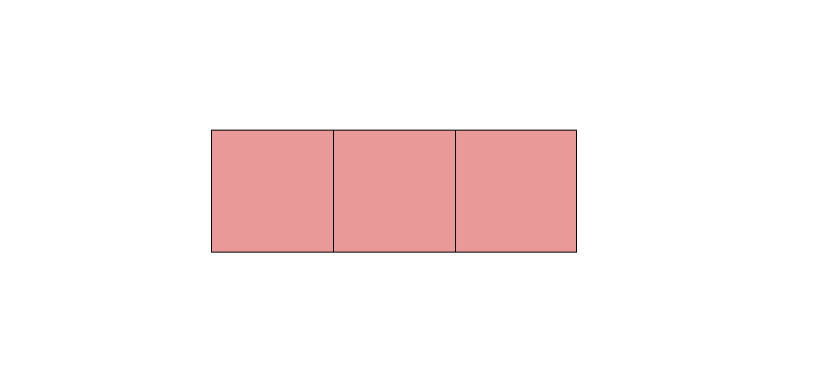
\includegraphics[width=5cm]{3x1}
\centering
\end{figure}
\\
\indent
Inductive Hypothesis: Assume any rectangle of dimension $3 \times n$, where $n$ is odd and $\leq 2k+1$, \textit{cannot} be covered exactly with L-shaped tiles.\\

Inductive Case: We can represent any rectangle where $n$ is odd as a rectangle where $n$ is even plus the non-tileable $3 \times 1$ rectangle. The even region will be exactly tileable as proven above, meaning no L-tiles can overlap with both the "even" and "odd" regions. \\

Similar to above if we consider a rectangle with dimension $3 \times 2(k+1) + 1 = 3 \times (2k+3)$ it will be the same as adding a $3 \times 2$ rectangle onto the existing one. This addition is exactly tileable as well and will not have any tiling overlap with the $3 \times 1$ portion. Because only exactly tileable regions will be added, this remainder portion can never be covered, therefore no $3 \times n$ rectangle where $n$ is odd can be completely covered with L-tiles. \\




\newpage
\section*{\textbf{6: P4.11.3} [12 pts]}
Prove the claim at the end of the section about the Euclidean Algorithm and Fibonacci numbers. Specifically, prove that if positive naturals $a$ and $b$ are each at most $F(n)$, then the Euclidean Algorithm performs at most $n - 2$ divisions. (You may assume that $n > 2$.) (It follows from this result that Fibonacci numbers are the worst case, but you may not use this fact to solve this problem!)



\subsection*{\textbf{Solution:}}
Proof by Induction:\\

Base Case: $n=3, $ F(3) = 2, $a$ and $b$ are at most 2, so the Euclidean algorithm will terminate in one step. $1 \leq 3-2$\\

Inductive Hypothesis: Assume the Euclidean Algorithm for $a$ and $b$ which are at most $F(k)$ terminates in at most $k-2$ steps for some $k \geq 3$.\\

Inductive Case: Let $a$ and $b$ be positive integers which are at most $F(k+1)$. Assume $a > b$. The first step of the EA will compute $a mod b$ which is at most $F(k+1)$ by our assumption. \\


\newpage
\section*{\textbf{7: P9.1.5} [10 pts]}
State and prove a theorem giving the maximum and minimum possible number of leaves in a rooted tree of depth $d$ and degree $k$. Repeat for the maximum and minimum total number of nodes.


\subsection*{\textbf{Solution:}}
Theorem 1:
\begin{enumerate}[a.]
	\item The maximum number of leaves in a rooted tree of depth $d$ and degree $k$ is $k^d$ (assuming the tree of one node has a depth of 0).
	\item The minimum number is $k$.
\end{enumerate} 

\noindent
Theorem 2: 
\begin{enumerate}[a.]
	\item The maximum number of total nodes in a rooted tree of depth $d$ and degree $k$ is $\dfrac{k^{d}-1}{k-1}$ (assuming the tree of one node has a depth of 1).
	\item The minimum number is $k+d$.
\end{enumerate}

\noindent
Proof of Theorem 1a:\\

Base Case: $d=0, k=k$, a tree with one node has 1 leaf. $k^0 = 1$\\

Inductive Hypothesis: Assume all rooted trees of depth $d \leq D$ and degree $k$ have a maximum number of leaves $k^d$.\\

Inductive Case: Suppose we construct a new tree $T$ with root node $r$ and $k$ subtrees $T_1, T_2 ,\cdots , T_k$. Assume these subtrees have a degree of $k$ and a depth of $D$. The new tree will have a depth of $D+1$ because the root adds an extra level. The total number of leaves will be the sum of the number of leaves in the subtrees. By our hypothesis we know they each have $k^D$ leaves so the total number of leaves in $T$ is:
\[ k^D + k^D + \cdots = k*k^D\]
Our expected number of leaves should be:
\[ k^{D+1} =  k*k^D \]
Thus the max number of leaves in a rooted tree of depth $d$ and degree $k$ is $k^d$.\\

\noindent
Proof of Theorem 1b:\\
The minimum requirement for a tree to be of depth $d$ is for some subtree to reach this depth. With nodes extending from the root with only one child each, we can reach this depth. Then we must split the last node into $k$ children to keep the $k$ degree property. So the minimum number of leaves is $k$.\\

\noindent
Proof of Theorem 2a: \\

The maximum number of nodes in a tree with depth $d$ and degree $k$ will occur in a full tree where all subtrees reach depth $d$ and all nodes have $k$ children. By this definition each level of the tree will have $k^d$ nodes where $d$ is the current depth level. Summing all of these nodes will give:
\[ k^0 + k^1 + k^2 + \cdots + k^d \]
This is a geometric series and can be represented as:
\[ \dfrac{k^{d}-1}{k-1} \]
Thus this is the maximum number of nodes in the tree.\\

\noindent
Proof of Theorem 2b:\\
We can use the exact same tree constructed in part 1b. This method will give us a tree of degree $k$ and depth $d$ with the least amount of nodes. If we add up the total number it will be $d$ nodes plus the leaves which is $k$ so $k+d$ nodes.


\newpage
\section*{\textbf{8: P9.3.5} [10 pts]}
Let $T$ be a parse tree for an expression with only unary and binary operators, and let $m$ be the number of primitive elements in the expression. Prove that if $m > 1$, then there exists a node $x$ of $T$ such that the subtree rooted at $x$ contains at least $m/3$ of the primitive elements and at most $2m/3$ of the primitive elements.


\subsection*{\textbf{Solution:}}
Proof by Induction:\\

Base Case: If we have a tree $T$ where $m=2$ the condition is satisfied because either subtree contains one primitive element which is between $\dfrac{2}{3}$ and $\dfrac{4}{3}$.\\

Inductive Hypothesis: Assume the condition above is satisfied for all parse trees with less than $m$ primitive elements.\\

Inductive Case: Suppose we have a tree $T$ with $m$ primitive elements. The number of primitive elements in the left subtree will be $m_1$ and in the right $m_2$. If $m_1 \geq m/3$ then the left subtree satisfies the condition, and we can choose $x$ as a node in the left subtree. If $m_2 \geq m/3$, then the right subtree satisfies the condition, and we can choose $x$ as a node in the right subtree. 



\newpage
\section*{\textbf{9: P9.4.7} [12 pts]}
Following Exercise 9.4.9, describe the state graph of the Towers of Hanoi puzzle for general $n$. Prove that the puzzle is always solvable, and find the number of moves in the shortest possible solution. (It will be useful to have a recursive definition of the state space.)


\subsection*{\textbf{Solution:}}
The Tower of Hanoi state graph resembles the Sierpiński triangle fractal, an equilateral triangle made up of recursive equaliteral triangles internally. Each node within this shape represents a state and the edges between them represent one move to change from one state to the other. This graph is not directed because moves can always be reversed. Take the base case for example of $n=1$. This will simply be a triangle with a node on each point representing the three possible places the one disk can be. All of these states are within one move of each other and are connected.\\

\noindent
To create a state graph for $n+1$, we take the original state graph and connect it by its corners to two other graphs of the same dimension, now giving us a larger triangle constructed by these triangles. (Note that the states themselves will change because there's now an additional disk to account for).\\

\noindent
When generalizing to higher values of $n$, it will always be true that the point nodes of the overall triangle represent the entire stack on each respective peg. With this in mind, it's easy to see that the shortest solution will always be the straight path along the edge of the triangle from the state with the entire stack on the left peg, to the state with the entire stack on the right peg (the goal state). Note that there will be a series of moves along this route that solve the puzzle. By our definition of how this graph recursively grows, we know the puzzle is always solvable because there will always exist a path between these two corner points.\\

\noindent
Proof by Induction that the puzzle is always solvable:\\

Base Case: $n = 1$, we know the Hanoi puzzle is trivially solvable with just one disk because we can just move it to the end in one move.\\

Inductive Hypothesis: Assume a Tower of Hanoi puzzle with number of disks $n$ is solvable for all values $k \leq n$, ($k \geq 1$). \\

Inductive Step: If we want to solve a Hanoi puzzle with $n+1$ disks we must move the first $n$ disks to the middle peg, then the $n+1$-th disk to the end, then the $n$ disks back onto the bigger one. By our hypothesis we know the puzzle is solvable for $n$ disks, therefore we know we can move them to the center because this would be the same as changing the center peg to the goal and the end peg to the helper/auxilliary. We also know we can move them back onto the largest disk at the end because it's again the same algorithm but using the end as the goal and left peg as the helper. Thus any Tower of Hanoi puzzle can be solved by moving the first $n-1$ disks, moving the $n$-th disk, then moving the $n-1$ disks again.\\\\\\

\noindent
Proof by Induction that the shortest number of moves is $2^n-1$:\\

Base Case: $n = 1$, $2^1-1=1$ move, as shown above one disk takes one move.\\

Inductive Hypothesis: Assume a Tower of Hanoi puzzle with number of disks $n$ can be solved in $2^n-1$ moves for all values $k \leq n$, ($k \geq 1$). \\

Inductive Step: If we evaluate the hypothesis for $n+1$ we get:
\[ 2^{n+1}-1 = 2*2^n-1\]
Let's now look at the moves in the puzzle itself using the solution method described above. Moving the first $n$ disks to the center takes $2^n-1$ moves by our hypothesis. Moving the largest disk to the end will take 1 move. And again moving the first $n$ disks back onto the largest disk on the last peg will take another $2^n-1$ moves.
\[ 2^n-1 + 1 + 2^n-1 = 2^n + 2^n - 1 = 2*2^n - 1 \]
Therefore the shortest number of moves to solve any Hanoi puzzle is $2^n-1$ moves.

\newpage
\section*{\textbf{EC: P9.5.8} [10 pts]}
In the knight’s tour problem, we are looking for a path of knight’s moves from a square of the $n \times n$ chessboard to itself, such that the path visits all $n^2$ squares of the board. How can we modify BFS or DFS to solve this problem? (The solution may not be efficient, but it is correct.)


\subsection*{\textbf{Solution:}}
We can first start with our starting square and perform a BFS from its location. This algorithm will use a queue to track the squares to move and search from as an open list. It will also use a closed list to track the squares already visited by the knight. We can continue to perform a BFS from each square that can be reached by a valid knight move from the previous square.\\

\noindent
The modification comes with how we use the closed list. If the newly popped node from the queue is in the closed list, it means the knight has already visited it and we don't need to check it again because its neighbors* are either already in the open list or have been checked already. This will remove the chance of the knight getting stuck in a cycle causing the algorithm to never terminate.\\

\noindent
We now continue to move to only unchecked squares. If the knight reaches a square at which all neigbors are already in the closed list, it must move backwards on its path to a square where this is not the case. We continue this process until all squares are in the closed list (meaning the knight has completed its tour) or all possible paths have been checked, in which case the knight's tour would be deemed impossible from our starting square on the given $n \times n$ board size.\\

*Consider a "neighbor" in this case to be any square the knight can move to from its current square.


\end{document} 